\documentclass[../main.tex]{subfiles}

\begin{document}

\problem{14}
Construct a nondeterministic finite-state automaton that recognizes the language generated by the regular grammar $G = (V, T, S, P)$, where $V = \{0, 1, S, A, B\}$, $T = \{0, 1\}$, $S$ is the start symbol, and the set of productions is
\begin{enumerate}[a)]
	\item $S \rightarrow 0A$, $S \rightarrow 1B$, $A \rightarrow 0$, $B \rightarrow 0$.
	\setcounter{enumi}{2}
	\item $S \rightarrow 1B$, $S \rightarrow 0$, $A \rightarrow 1A$, $A \rightarrow 0B$, $A \rightarrow 1$, $A \rightarrow 0$, $B \rightarrow 1$.
\end{enumerate}

\solution
\begin{enumerate}[a)]
	\item \hfill
\begin{center}
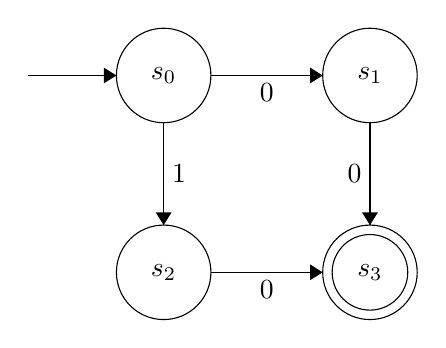
\begin{tikzpicture}[scale=0.2]
\tikzstyle{every node}+=[inner sep=0pt]
\draw [black] (13,-20.2) circle (3);
\draw (13,-20.2) node {$s_0$};
\draw [black] (26.1,-20.2) circle (3);
\draw (26.1,-20.2) node {$s_1$};
\draw [black] (13,-32.7) circle (3);
\draw (13,-32.7) node {$s_2$};
\draw [black] (26.1,-32.7) circle (3);
\draw (26.1,-32.7) node {$s_3$};
\draw [black] (26.1,-32.7) circle (2.4);
\draw [black] (4.4,-20.2) -- (10,-20.2);
\fill [black] (10,-20.2) -- (9.2,-19.7) -- (9.2,-20.7);
\draw [black] (13,-23.2) -- (13,-29.7);
\fill [black] (13,-29.7) -- (13.5,-28.9) -- (12.5,-28.9);
\draw (13.5,-26.45) node [right] {$1$};
\draw [black] (16,-32.7) -- (23.1,-32.7);
\fill [black] (23.1,-32.7) -- (22.3,-32.2) -- (22.3,-33.2);
\draw (19.55,-33.2) node [below] {$0$};
\draw [black] (26.1,-23.2) -- (26.1,-29.7);
\fill [black] (26.1,-29.7) -- (26.6,-28.9) -- (25.6,-28.9);
\draw (25.6,-26.45) node [left] {$0$};
\draw [black] (16,-20.2) -- (23.1,-20.2);
\fill [black] (23.1,-20.2) -- (22.3,-19.7) -- (22.3,-20.7);
\draw (19.55,-20.7) node [below] {$0$};
\end{tikzpicture}
\end{center}
	\setcounter{enumi}{2}
	\item \hfill
\begin{center}
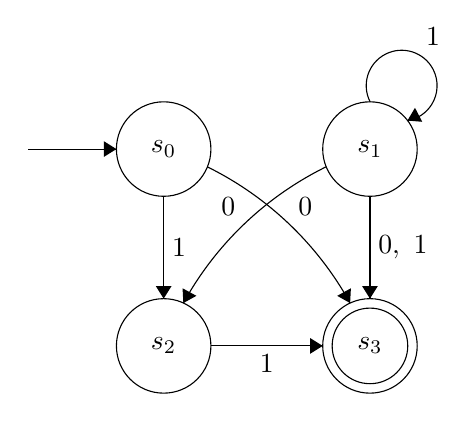
\begin{tikzpicture}[scale=0.2]
\tikzstyle{every node}+=[inner sep=0pt]
\draw [black] (13,-20.2) circle (3);
\draw (13,-20.2) node {$s_0$};
\draw [black] (26.1,-20.2) circle (3);
\draw (26.1,-20.2) node {$s_1$};
\draw [black] (13,-32.7) circle (3);
\draw (13,-32.7) node {$s_2$};
\draw [black] (26.1,-32.7) circle (3);
\draw (26.1,-32.7) node {$s_3$};
\draw [black] (26.1,-32.7) circle (2.4);
\draw [black] (4.4,-20.2) -- (10,-20.2);
\fill [black] (10,-20.2) -- (9.2,-19.7) -- (9.2,-20.7);
\draw [black] (13,-23.2) -- (13,-29.7);
\fill [black] (13,-29.7) -- (13.5,-28.9) -- (12.5,-28.9);
\draw (13.5,-26.45) node [right] {$1$};
\draw [black] (16,-32.7) -- (23.1,-32.7);
\fill [black] (23.1,-32.7) -- (22.3,-32.2) -- (22.3,-33.2);
\draw (19.55,-33.2) node [below] {$1$};
\draw [black] (26.1,-23.2) -- (26.1,-29.7);
\fill [black] (26.1,-29.7) -- (26.6,-28.9) -- (25.6,-28.9);
\draw (26.6,-26.45) node [right] {$0,\mbox{ }1$};
\draw [black] (15.776,-21.331) arc (63.73967:28.94558:20.952);
\fill [black] (24.84,-29.98) -- (24.89,-29.04) -- (24.02,-29.52);
\draw (21.99,-24.48) node [above] {$0$};
\draw [black] (14.254,-29.977) arc (151.14948:116.16527:20.849);
\fill [black] (14.25,-29.98) -- (15.08,-29.52) -- (14.2,-29.04);
\draw (17.1,-24.47) node [above] {$0$};
\draw [black] (26.116,-17.212) arc (207.43495:-80.56505:2.25);
\draw (30.11,-13.66) node [above] {$1$};
\fill [black] (28.48,-18.39) -- (29.42,-18.47) -- (28.96,-17.58);
\end{tikzpicture}
\end{center}
\end{enumerate}

\end{document}
